\beginsong{Die freie Republik}[wuw={Studentengruppen, Januar 1937}, bo={206}, pfii={47}, pfiii={23}, gruen={183}, kssiv={22}, index={In dem Kerker saßen}]

\beginverse
\endverse
\centering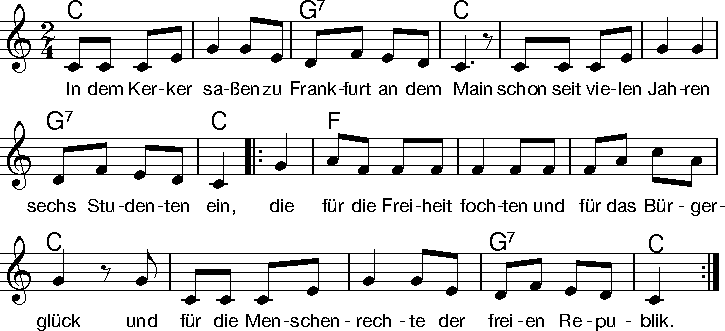
\includegraphics[width=1\textwidth]{Noten/Lied022.pdf}	

\beginverse
\[C]Und der Kerkermeister \[G7]sprach es täglich \[C]aus:
''Sie, Herr Bürgermeister, es \[G7]reißt mir keiner \[C]aus!''
\lrep Aber \[F]doch sind sie verschwunden abends aus dem \[C]Turm,
um die zwölfte Stunde, \[G7]bei dem großen \[C]Sturm. \rrep
\endverse

\beginverse
^Und am ander'n Morgen ^hört man den A^larm.
Oh, es war entsetzlich, ^der Soldaten^schwarm!
\lrep Sie ^suchten auf und nieder, sie suchten hin und ^her,
sie suchten sechs Studenten und ^fanden sie nicht ^mehr. \rrep
\endverse

\beginverse
^Doch sie kamen wieder, mit ^Schwertern in der ^Hand.
''Auf, auf, ihr deutschen Brüder, jetzt ^geht's für's Vater^land!
\lrep Jetzt ^geht's für Menschenrechte und für das Bürger^glück!
Wir sind doch keine Knechte der ^freien Repu^blik.'' \rrep
\endverse

\beginverse
^Wenn euch die Leute fragen: ''^Wo ist Absa^lom?''
So dürfet ihr wohl sagen: ''^Oh, der hänget ^schon.''
\lrep Er ^hängt an keinem Baume, er hängt an keinem ^Strick,
sondern an dem Glauben an die ^freie Repu^blik. \rrep
\endverse


\endsong

\beginscripture{}
Erkennungslied der demokratischen Bewegung zu jener Zeit. Text und Musik entstanden nach der Befreiung von 6 Studenten, die mit dem Frankfurter Wachensturm (auf die Hauptwache und die Konstablerwache) vom 3. April 1833 versucht hatten, eine Revolution auszulösen. Ihre Flucht gelang schließlich mit Hilfe der Gefangenenwärter. In Folge dieser Verschwörung wurden mehr als 1.800 Personen zur Fahndung ausgeschrieben und 39 Personen zum Tod oder zu lebenslanger Haft verurteilt.
\endscripture
